\documentclass[11pt,a4paper,DIV20]{scrartcl}
\usepackage{amsmath}
\usepackage{amssymb}
\usepackage{graphicx}
\usepackage{multicol}
\usepackage[compat=1.1.0]{tikz-feynman}
\usetikzlibrary{shapes}

\title{Diagrams (total \# 1)\\[-0.5em]}
\author{\ttfamily{Richard\_Draw.py}}
\date{}

\begin{document}
\maketitle
\centering
\begin{verbatim}
----------------------------------------------------
 output = 'diagrams.dat' ;
 style = '../../richard_draw.sty' ;
 model = '../standardmodel.lag' ;
 in = fd[q1];
 out = fd[q2];
 loops = 1 ;
 loop_momentum = p ;
 options = onshell,tadpole;
 true = iprop[a,g,G0,0,0];
 true = iprop[h,1,1];
 true = iprop[ft,1,1];
----------------------------------------------------
\end{verbatim}
\begin{minipage}[]{0.32\textwidth}
\begin{center}
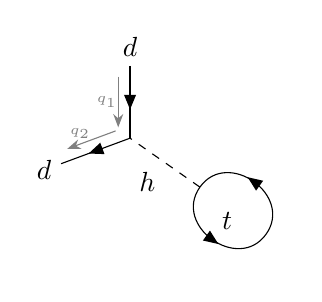
\begin{tikzpicture}
\tikzfeynmanset{}
\begin{feynman}
\diagram[small]{
   i1 [particle=$d$] -- [fermion, momentum'={[arrow style=gray, label distance=-1mm, arrow distance=1.5mm] {\tiny $q_{1}$}}] v1,
   v1 -- [fermion, momentum'={[arrow style=gray, label distance=-1mm, arrow distance=1.5mm] {\tiny $q_{2}$}}] o2 [particle=$d$], 
   v2 -- [half right, edge label=$t$, fermion] t2,
   t2 -- [half right, fermion] v2,
   v2 -- [edge label=$h$, scalar] v1,
};
\end{feynman}
\end{tikzpicture}\\
\# $1$ \\
(symmetry: $-1$)
\end{center}
\end{minipage}
%
\end{document}
